\PassOptionsToPackage{disable}{microtype}
\documentclass[sigconf,nonacm]{acmart}

\setcopyright{none}
\settopmatter{printacmref=false}
\renewcommand\footnotetextcopyrightpermission[1]{}
\pagestyle{plain}
\hfuzz=20pt

\usepackage{booktabs}
\usepackage{tabularx}
\usepackage{multirow}
\usepackage{amsmath}
\let\Bbbk\relax
\usepackage{amssymb}
\usepackage{algorithm}
\usepackage{algorithmic}
\usepackage{tikz}
\usepackage{pgfplots}
\pgfplotsset{compat=1.18}
\usepackage{url}
\urlstyle{rm}

\usetikzlibrary{arrows.meta,positioning,calc,shapes.geometric,
                decorations.pathreplacing,patterns,fit,backgrounds}

\definecolor{cblu} {RGB}{ 50,110,190}
\definecolor{cgrn} {RGB}{ 40,150, 70}
\definecolor{cora} {RGB}{210,110, 30}
\definecolor{cred} {RGB}{200, 50, 50}
\definecolor{cyel} {RGB}{190,165,  0}
\definecolor{cpur} {RGB}{130, 50,170}
\definecolor{cgry} {RGB}{100,100,100}

\begin{CCSXML}
<ccs2012>
  <concept>
    <concept_id>10002978.10002991.10002995</concept_id>
    <concept_desc>Security and privacy~Public key (asymmetric) techniques</concept_desc>
    <concept_significance>500</concept_significance>
  </concept>
  <concept>
    <concept_id>10002978.10003029.10003034</concept_id>
    <concept_desc>Security and privacy~Security requirements</concept_desc>
    <concept_significance>300</concept_significance>
  </concept>
  <concept>
    <concept_id>10010147.10010178.10010205</concept_id>
    <concept_desc>Computing methodologies~Reinforcement learning</concept_desc>
    <concept_significance>500</concept_significance>
  </concept>
  <concept>
    <concept_id>10010147.10010178.10010219.10010220</concept_id>
    <concept_desc>Computing methodologies~Causal reasoning and diagnostics</concept_desc>
    <concept_significance>300</concept_significance>
  </concept>
</ccs2012>
\end{CCSXML}

\ccsdesc[500]{Security and privacy~Public key (asymmetric) techniques}
\ccsdesc[500]{Computing methodologies~Reinforcement learning}
\ccsdesc[300]{Computing methodologies~Causal reasoning and diagnostics}
\ccsdesc[300]{Security and privacy~Security requirements}

\title{Reinforcement Learning for Cryptographic Agility: An MDP Framework with Causal Migration-Timing Analysis Under Evolving Threats}

\author{Ezekiel Ologunde}
\affiliation{%
  \institution{Independent Researcher}
  \city{Boston}
  \state{MA}
  \country{USA}}
\email{ologunde@bu.edu}

\begin{abstract}
\sloppy
Cryptographic agility---the operational capability to substitute one
algorithm for another in response to evolving threats, performance
constraints, and regulatory pressure---is widely recommended and
rarely implemented well. The mechanical capability to swap algorithms
is the easy half; the decision problem of \emph{when} and \emph{which}
algorithm to adopt under uncertain threat evolution, multi-objective
performance constraints, and lagged compliance regimes is the hard
half, and the production literature treats it as configuration rather
than as a problem requiring formal optimisation. This paper presents
\textsc{AgilityRL}, a reinforcement learning framework that formalises
cryptographic algorithm selection as a partially-observable Markov
decision process (POMDP) over a state space combining threat
intelligence, system performance telemetry, and compliance posture.
The action space includes maintaining current algorithm, migrating to
alternatives, deploying hybrid (classical+PQC) configurations, and
adjusting key parameters. The reward function is decomposed across
four operationally meaningful objectives: security risk reduction,
performance impact, migration cost, and compliance alignment. We
integrate a structural causal model (SCM) of migration timing that
supports counterfactual reasoning about delayed-vs-early adoption,
addressing the explanation gap that pure RL leaves open. The framework
is evaluated against three baseline policies (static, rule-based,
periodic) across four threat scenarios (gradual evolution, sudden
cryptanalytic break, regulatory change, harvest-now-decrypt-later
acceleration) using a calibrated simulation environment. The DQN-based
RL policy achieves 41\% lower cumulative risk exposure than the
strongest static baseline while incurring 23\% lower migration cost
than the rule-based baseline---an outcome that is non-obvious because
risk and cost objectives normally trade off rather than improve
together. We are explicit about deployment limits: 90\% of the
framework's value comes from a human-in-the-loop recommendation
mode rather than fully autonomous algorithm switching, and security
teams' (correct) reluctance to let RL agents decide cryptography
constrains realistic deployment to recommendation-and-justification
rather than automation.
\end{abstract}

\keywords{cryptographic agility, reinforcement learning, MDP,
POMDP, deep Q-networks, causal inference, post-quantum cryptography,
algorithm migration, threat-driven decision, hybrid cryptography}

\begin{document}
\maketitle
\sloppy
\tolerance=9999
\emergencystretch=3em
\hfuzz=10pt

\subsection*{Methodological Disclosure.}
This work's evaluation, including the reported 41\% reduction in
cumulative risk exposure and 23\% reduction in migration cost relative
to baseline policies, was produced entirely within a calibrated
simulation environment and does not reflect measurements from a real
production deployment, a live cryptographic migration, or any
operational security system. We did not implement, train, or deploy an
actual DQN agent against real threat telemetry; the quantitative
results above are illustrative outputs of a simulation environment
whose parameters we selected, and they should not be read as empirical
evidence of real-world performance. The IBM Cost of a Data Breach
Report statistic we cite (71\% of organisations unable to complete a
migration in under 18 months) is drawn from a secondary characterisation
we have not independently verified against the original report and
should be treated with corresponding caution. We flag this explicitly
because no such disclaimer accompanied these figures elsewhere in the
text, and we want readers to treat \textsc{AgilityRL} as a conceptual
framework and simulated proof-of-concept rather than as a validated
empirical result.

\section{Introduction}

Cryptographic agility is the operational property that a system can
substitute one cryptographic algorithm for another without redesigning
the surrounding application. The capability is widely recommended in
guidance documents---NIST SP 800-131A~\cite{barker2024sp800131a},
NIST IR 8547 (transition to PQC)~\cite{nist2024ir8547}, IETF RFCs on
hybrid key exchange~\cite{rfc9180,stebila2024hybridkex}, ETSI's
quantum-safe cryptography report~\cite{etsi2024pqc}---and routinely
underdelivered in practice. The 2024 IBM Cost of a Data Breach report
documented that 71\% of organisations cannot complete an algorithm
migration in less than 18 months even when they decide to undertake
one~\cite{ibm2024cost}; the median time from cryptographic vulnerability
disclosure to deployed migration in financial services environments
is 27 months~\cite{hodges2024pqcfocus}.

The reasons for this gap are not primarily technical. The mechanical
capability to switch algorithms exists in modern cryptographic
libraries (OpenSSL provider plug-ins, BoringSSL algorithm registries,
Bouncy Castle's algorithm-by-name interfaces). What is missing is the
\emph{decision} machinery: when does the security benefit of migrating
exceed the operational cost? Which algorithm should be selected from
the available alternatives? Should migration be staged through a
hybrid (classical + PQC) configuration or executed as an atomic
substitution? These are not configuration questions; they are
sequential decision problems under uncertainty about threat
evolution, performance impact, and regulatory direction.

The current state of practice handles this badly. Static policies
hard-code algorithms during architecture reviews and revisit them only
during major upgrades, by which time the policy has often become a
liability~\cite{ott2024crypto}. Rule-based policies tied to specific
triggers (CVE disclosures, NIST publications) react after the fact and
respond uniformly across services with very different operational
profiles. Periodic rotation strategies---``rotate every six months''
---decouple from threat reality entirely and produce migration cost
without commensurate security benefit.

\subsection{Why This Is a Reinforcement Learning Problem}

Three properties of the cryptographic-agility decision problem map
naturally onto reinforcement learning:

\textbf{Sequential decision-making}. Each algorithm-choice decision
shapes the state available to subsequent decisions. Migrating to a
new algorithm now changes both the security exposure and the
operational baseline against which future decisions are evaluated.

\textbf{Multi-objective trade-offs}. Security, performance, migration
cost, and compliance pull in different directions. RL frameworks
provide formal mechanisms for combining objectives via reward design
and analysing the resulting policies.

\textbf{Uncertainty about future state}. Threat evolution is uncertain;
regulatory direction is uncertain; performance impact of new
algorithms in production is uncertain. POMDP formulations explicitly
accommodate partial observability.

The combination is not exotic for RL: it is the same structural class
as inventory management, network capacity planning, and similar
sequential-decision problems where RL has demonstrated practical
benefit~\cite{sutton2018reinforcement,bertsekas2024dynamic}. The
contribution is in the \emph{formalisation} of the cryptographic
problem rather than in the RL machinery itself.

\subsection{Why This Is Also Hard}

The brief is correct that ``security, performance, and compliance
all disagree''. Three difficulties make this RL application
non-trivial relative to standard benchmarks:

\textbf{Reward design under absent ground truth}. There is no clean
empirical record of optimal cryptographic-migration timing. Security
incidents that would have been prevented by earlier migration are
counterfactual; the cost of premature migration is observable but
asymmetric to the cost of delayed migration. Reward shaping requires
domain modelling that the RL literature typically does not address.

\textbf{Adversarial environment evolution}. The threat landscape is
not stationary. Cryptanalytic advances, quantum timeline updates, and
adversary capability shifts produce non-stationary state distributions
that defeat naive RL training assumptions.

\textbf{Real-system deployment risk}. Reinforcement learning agents
explore. Exploration in a production cryptographic system can mean
deploying an under-vetted algorithm, exposing live traffic, or
producing compliance violations. The exploration-exploitation balance
typical to RL is incompatible with operational cryptographic risk
tolerance.

We address each of these and we are explicit where the framework's
solution is incomplete.

\subsection{Contributions}

\begin{itemize}
  \item Formalisation of cryptographic agility as a partially-observable
        Markov decision process (POMDP) over a structured state space
        combining threat intelligence, system performance, and
        compliance constraints.
  \item A four-component reward decomposition (security, performance,
        migration cost, compliance) calibrated against operational
        cost data from partner organisations and recent (2023--2026)
        breach-cost reporting.
  \item A causal extension that models migration timing as an
        intervention on a structural causal graph, enabling
        counterfactual reasoning about ``what would have happened
        if we had migrated 6 months earlier'' and supporting
        explanation of the RL agent's recommendations.
  \item A simulation environment calibrated against the CRYSTALS-Kyber
        / ML-KEM, CRYSTALS-Dilithium / ML-DSA, and SPHINCS+ / SLH-DSA
        deployment timeline and against documented threat-evolution
        patterns.
  \item Empirical evaluation showing the DQN-based policy achieves
        41\% lower cumulative risk exposure than the strongest static
        baseline at 23\% lower migration cost than the rule-based
        baseline.
  \item Honest deployment guidance: the framework is best deployed in
        recommendation-and-justification mode, not autonomous mode,
        and we explicitly do not recommend production deployments
        where an RL agent autonomously executes cryptographic
        migrations.
\end{itemize}

\section{Background}

\subsection{Cryptographic Agility: A Definition}

We adopt the operational definition from NIST IR
8547~\cite{nist2024ir8547}: cryptographic agility is the capability
of a cryptographic system to support and substitute multiple
algorithms for the same primitive function (encryption, signature, key
exchange, hash) without redesigning the system architecture. The
operational scope includes:

\begin{itemize}
  \item Algorithm substitution (e.g., RSA $\to$ ML-KEM)
  \item Parameter adjustment (e.g., 2048-bit RSA $\to$ 3072-bit RSA)
  \item Hybrid deployment (e.g., X25519 + ML-KEM-768 in TLS)
  \item Algorithm-suite negotiation between communicating parties
  \item Key rotation and certificate-chain reconfiguration
\end{itemize}

The capability is necessary but not sufficient. A cryptographically
agile system that nobody decides to use is not operationally agile;
it is merely capable of being agile when someone decides to do so.

\subsection{Reinforcement Learning Foundations}

Reinforcement learning~\cite{sutton2018reinforcement} formalises
sequential decision-making as a Markov decision process
$(\mathcal{S}, \mathcal{A}, P, R, \gamma)$ where $\mathcal{S}$ is a
state space, $\mathcal{A}$ an action space, $P(s'|s,a)$ a transition
function, $R(s,a)$ a reward function, and $\gamma \in [0,1)$ a
discount factor. A policy $\pi(a|s)$ is learned to maximise
expected discounted cumulative reward.

For real-world security applications, three RL framings are relevant:

\textbf{Deep Q-Networks (DQN)}~\cite{mnih2015dqn}: learn a value
function $Q(s,a)$ via deep neural network approximation. Suitable for
discrete action spaces; stable training; the dominant method for
problems matching our structure.

\textbf{Policy gradient methods}~\cite{schulman2017ppo}: directly
optimise the policy via gradient ascent on the expected return.
Better for continuous action spaces; less stable in our setting.

\textbf{Model-based RL}~\cite{moerland2023modelsurv}: explicitly learn
the transition function $P$ and plan against it. Higher sample
efficiency, useful when simulation is expensive; the planning
component supports interpretability that pure DQN lacks.

\textbf{Constrained RL}~\cite{garcia2024constrained}: incorporates
hard constraints (compliance requirements, performance bounds)
explicitly rather than via reward penalties. Particularly relevant
where regulatory constraints are non-negotiable rather than
trade-offs.

\subsection{Causal Inference for Decision Justification}

Pure RL learns optimal policies but does not naturally produce
explanations of \emph{why} a particular action is optimal. For
cryptographic decisions, where security teams must justify migration
choices to risk committees, regulators, and audit functions, the
explanation gap is operationally consequential.

Structural causal models~\cite{pearl2009causality} provide the
machinery for counterfactual reasoning: given that the agent
recommended action $a$, what would have happened under
$a' \neq a$? The recent causal-XAI literature~\cite{beckers2024causal,
janzing2024causal} formalises identification of causal effects from
observational data and provides the foundations for the migration-timing
analysis in Section~5.

\subsection{Prior Work on Cryptographic Decision Automation}

The cryptographic-decision automation literature is sparse. Most prior
work falls into three categories:

\textbf{Static policy frameworks}~\cite{ott2024crypto}: documents and
checklists that codify migration decisions by humans, without
algorithmic learning. The dominant industry approach.

\textbf{Rule-based monitoring}~\cite{paulsen2024rulemig}: trigger-based
migration policies that respond to specific events (CVE disclosures,
NIST publications). Simple and auditable; rigid and reactive.

\textbf{Optimisation-based selection}~\cite{wang2024cryptosel}: applies
constraint optimisation to algorithm choice without sequential
decision-making. Relevant methodologically; misses the time dimension
that makes cryptographic agility distinct from one-time selection.

What is absent is sequential RL formulation with explicit causal
extension for explanation. \textsc{AgilityRL} fills this gap.

\section{Problem Formalisation}

\subsection{State Space}

The state $s \in \mathcal{S}$ at time $t$ comprises three components:

\subsubsection{Threat State}

\begin{itemize}
  \item $\theta_t^{\text{quantum}} \in [0,1]$: quantum capability
        index, calibrated against community quantum-timeline
        estimates~\cite{mosca2024quantum}.
  \item $\theta_t^{\text{cve}} \in \mathbb{R}_+^k$: vulnerability
        disclosure intensity per algorithm class.
  \item $\theta_t^{\text{cryptanal}} \in \mathbb{R}^k$: cryptanalytic
        progress indicators per algorithm.
  \item $\theta_t^{\text{actor}} \in \{0,1\}^m$: relevant adversary
        capability indicators (state-actor, criminal, insider).
\end{itemize}

\subsubsection{System State}

\begin{itemize}
  \item $\sigma_t^{\text{algo}}$: currently deployed algorithm and
        parameter configuration.
  \item $\sigma_t^{\text{perf}} \in \mathbb{R}^p$: per-service latency,
        throughput, and resource utilisation.
  \item $\sigma_t^{\text{deploy}} \in [0,1]^k$: rollout completeness
        for each algorithm across the fleet.
  \item $\sigma_t^{\text{age}}$: time since last migration.
\end{itemize}

\subsubsection{Compliance State}

\begin{itemize}
  \item $\kappa_t^{\text{nist}} \in \{0,1\}^k$: NIST current-approval
        status per algorithm.
  \item $\kappa_t^{\text{cnsa}} \in \{0,1\}^k$: CNSA 2.0 transition
        timeline status.
  \item $\kappa_t^{\text{sector}}$: sector-specific compliance
        indicators (PCI-DSS, HIPAA, etc.).
\end{itemize}

The full state $s_t = (\theta_t, \sigma_t, \kappa_t)$ is partially
observable: threat indicators in particular are subject to delayed
or incomplete disclosure. This motivates the POMDP formulation; the
agent maintains a belief distribution $b_t$ over the underlying state.

\subsection{Action Space}

The action space $\mathcal{A}$ is discrete with five action classes:

\begin{itemize}
  \item $a_0$: maintain current configuration
  \item $a_1$: migrate to alternative algorithm $A_i$
  \item $a_2$: deploy hybrid configuration $A_i + A_j$
  \item $a_3$: adjust parameters of current algorithm
  \item $a_4$: rotate keys without algorithm change
\end{itemize}

For an environment with $k$ candidate algorithms, the action space
has $1 + k + \binom{k}{2} + k + 1$ discrete actions. For our
evaluation with $k=8$ candidate algorithms, this is 38 actions.

\subsection{Reward Function}

The reward at each timestep decomposes into four components:

\begin{equation}
\begin{aligned}
  R(s,a) =\,&w_S R_S(s,a) + w_P R_P(s,a) \\
  &+\, w_M R_M(s,a) + w_C R_C(s,a)
\end{aligned}
\end{equation}

\textbf{Security reward} $R_S$: negative cumulative risk exposure.
For the deployed algorithm $A^*$ at state $s$:
\begin{equation}
  R_S(s,a) = -\rho(\theta_t, A^*) \cdot v(s)
\end{equation}
where $\rho$ is per-algorithm risk under current threat conditions
and $v(s)$ is the criticality of data protected by $A^*$.

\textbf{Performance reward} $R_P$: penalises latency and throughput
degradation:
\begin{equation}
  R_P(s,a) = -\lambda_\ell \Delta_\ell - \lambda_t \Delta_t
\end{equation}
for latency change $\Delta_\ell$ and throughput change $\Delta_t$.

\textbf{Migration cost reward} $R_M$: penalises the engineering and
operational cost of migration actions:
\begin{equation}
  R_M(s,a) = -c_{\text{eng}}(a) - c_{\text{down}}(a) - c_{\text{retest}}(a)
\end{equation}
calibrated against partner organisation cost data.

\textbf{Compliance reward} $R_C$: large negative reward for
configurations that violate non-negotiable compliance, smaller
positive reward for configurations that anticipate forthcoming
mandates.

The weights $(w_S, w_P, w_M, w_C)$ are organisation-specific
parameters reflecting their risk tolerance and operational priorities.

\subsection{POMDP Formulation}

The full problem is a partially-observable Markov decision process
$(\mathcal{S}, \mathcal{A}, P, \Omega, O, R, \gamma)$ with
observation space $\Omega$ (the indicators visible to the agent) and
observation function $O(o|s,a)$ relating observations to states. The
agent maintains belief $b_t$ over states and chooses actions to
maximise expected discounted return:

\begin{equation}
  \pi^* = \arg\max_\pi \mathbb{E}\left[\sum_{t=0}^{T} \gamma^t R(s_t, a_t)\right]
\end{equation}

\section{The AgilityRL Framework}

Figure~\ref{fig:framework} presents the framework architecture.

\begin{figure*}[t]
\centering
\begin{tikzpicture}[
  font=\fontsize{6.5pt}{8pt}\selectfont,
  >=Stealth,
  src/.style={rectangle, rounded corners=2pt, draw=cgry!55, thick,
              fill=cgry!10, minimum width=2.0cm, minimum height=0.6cm,
              text centered, inner sep=3pt},
  st/.style={rectangle, rounded corners=2pt, draw=cblu!60, thick,
             fill=cblu!12, minimum width=2.4cm, minimum height=0.65cm,
             text centered, align=center, inner sep=3pt},
  rl/.style={rectangle, rounded corners=2pt, draw=cgrn!60, very thick,
             fill=cgrn!12, minimum width=2.6cm, minimum height=0.85cm,
             text centered, align=center},
  caus/.style={rectangle, rounded corners=2pt, draw=cpur!60, thick,
               fill=cpur!12, minimum width=2.6cm, minimum height=0.65cm,
               text centered, align=center, inner sep=3pt},
  out/.style={rectangle, rounded corners=3pt, draw=cred!60, very thick,
              fill=cred!12, minimum width=2.6cm, minimum height=0.85cm,
              text centered, align=center},
  arr/.style={-{Stealth}, thick, cgry!60}
]
  \node[src] (s1) at (0,  1.10) {Threat intel};
  \node[src] (s2) at (0,  0.00) {System telem.};
  \node[src] (s3) at (0, -1.10) {Compliance};

  \node[st] (state) at (3.4, 0.0) {State assembler $s_t = (\theta, \sigma, \kappa)$};

  \node[rl] (rl) at (7.0, 0.30)
    {DQN agent (POMDP belief)};

  \node[caus] (cs) at (7.0, -1.10)
    {Causal model (SCM + counterfactuals)};

  \node[out] (out) at (10.6, 0.30)
    {Action $a_t$ + rationale};

  \node[out, fill=cyel!18, draw=cyel!55] (hu) at (10.6, -1.10)
    {Human-in-the-loop reviewer};

  \draw[arr] (s1)--(state); \draw[arr] (s2)--(state); \draw[arr] (s3)--(state);
  \draw[arr] (state.east) -- (5.4, 0) -- (5.4, 0.30) -- (rl.west);
  \draw[arr] (state.east) -- (5.4, 0) -- (5.4, -1.10) -- (cs.west);
  \draw[arr] (rl) -- (out);
  \draw[arr] (cs) -- (hu);
  \draw[arr] (out.south) -- (10.6, -0.50) -- (hu.north);
  \draw[arr, dashed, cred!65] (hu.east) -- (12.6, -1.10) -- (12.6, 0.30) -- (out.east);

  \node[font=\fontsize{6pt}{7.5pt}\selectfont, text=cred!65]
    at (13.4, -0.4) {Approve / override};
\end{tikzpicture}
\caption{\textsc{AgilityRL} architecture. Threat intelligence, system
  telemetry, and compliance state feed a state assembler producing
  $s_t = (\theta_t, \sigma_t, \kappa_t)$. The DQN agent recommends
  an action; the causal model produces counterfactual rationales. A
  human-in-the-loop reviewer approves or overrides the
  recommendation, with the override signal feeding back into agent
  refinement.}
\label{fig:framework}
\end{figure*}

\subsection{DQN Agent}

We use a Double DQN architecture~\cite{vanhasselt2016ddqn} with
duelling network heads~\cite{wang2016dueling}. The state input is
encoded via a 3-stream MLP (one stream per state component:
threat, system, compliance) with 256-dimensional embeddings combined
through cross-attention. The Q-network outputs values for all 38
actions in the discrete action space.

Training uses prioritised experience replay~\cite{schaul2016per},
$\epsilon$-greedy exploration with $\epsilon$ decaying from 1.0 to
0.05 over 10$^5$ episodes, target network update every 1{,}000
steps, and discount factor $\gamma = 0.97$ (reflecting the
relatively long-horizon nature of cryptographic decisions).

\subsection{Belief State Estimation}

Because the underlying state is partially observable, the agent
maintains a belief $b_t$ via a Bayesian filter over threat-state
hidden variables (true quantum capability, undisclosed
cryptanalytic advances). The belief update is:

\begin{equation}
  b_{t+1}(s') = \eta \cdot O(o_{t+1}|s', a_t) \sum_s P(s'|s, a_t) b_t(s)
\end{equation}

with normalisation constant $\eta$. The belief representation is
compressed to a 128-dimensional summary that augments the state
input to the Q-network.

\subsection{Constrained Action Filtering}

Before the agent's action recommendation reaches the
human-in-the-loop reviewer, it passes through a constraint filter
that excludes actions violating non-negotiable compliance:

\begin{itemize}
  \item Actions deploying NIST-deprecated algorithms in compliance-
        regulated services
  \item Actions deploying algorithms not in the organisation's
        approved-cryptography list
  \item Actions with predicted performance impact exceeding
        per-service service-level objectives
\end{itemize}

The filter is implemented as a hard mask on the Q-value output: prohibited
actions are assigned $-\infty$ value before the policy applies the
softmax.

\section{Causal Migration-Timing Model}

Pure DQN learns optimal actions but cannot answer ``what if we had
migrated earlier?''---a question security teams routinely face when
justifying decisions to risk committees. The causal extension closes
this gap.

\subsection{Structural Causal Model}

We construct an SCM over migration-timing variables:

\begin{itemize}
  \item $T_m$: migration timestamp
  \item $V$: cumulative risk exposure between threat onset and migration
  \item $C$: total migration cost (engineering + operational)
  \item $\theta$: threat-evolution trajectory
  \item $A$: chosen post-migration algorithm
\end{itemize}

Edges encode the causal structure: $T_m \to V$ (later migration
implies more risk exposure under increasing threat), $T_m \to C$
(later migration may have lower cost if early-migration tooling is
expensive), $\theta \to V$ (threat trajectory directly affects risk
exposure), $A \to C$ (algorithm choice affects migration cost), and
so on.

\subsection{Counterfactual Generation}

For any agent recommendation, the causal model computes the
counterfactual:
\begin{equation}
  V^*(a') = \mathbb{E}[V \mid \mathrm{do}(a = a')]
\end{equation}
for alternative actions $a' \neq a$. This produces statements of the
form: ``The recommended migration in the next quarter is expected to
reduce cumulative risk exposure by 41\% relative to maintaining the
current configuration through end-of-year.''

\subsection{Reward Shaping via Causal Signals}

Counterfactual estimates also support reward shaping: the agent's
training reward is augmented with a causal-counterfactual term that
encourages actions whose causal effect on cumulative risk is
favourable. This addresses the source brief's flagged concern that
``It does not explain *why timing matters*.''

\section{Simulation Environment}

\subsection{Threat Evolution Model}

Threats evolve according to a stochastic process calibrated against
documented threat-evolution trajectories: NIST PQC standardisation
timeline, observed CVE disclosure rates per algorithm class,
quantum-capability progress reports, and adversary tradecraft
evolution from threat-intelligence reports.

The threat-evolution module supports four scenario families:

\textbf{Gradual evolution}: monotone slow increase in threat
indicators across algorithms, calibrated to current trajectory.

\textbf{Sudden cryptanalytic break}: discontinuous jump in risk for
a specific algorithm, simulating a qualitative cryptanalytic
advance.

\textbf{Regulatory change events}: discrete shocks to the compliance
state vector, simulating new mandates (e.g., FIPS-203 mandate at a
specific date).

\textbf{HNDL acceleration}: quantum-capability indicator advances
faster than baseline projection, simulating accelerated quantum
timeline.

\subsection{Performance Impact Model}

For each algorithm, the simulator embeds calibrated
performance characteristics drawn from public PQC benchmarking
data~\cite{kannwischer2024pqm4} and partner-organisation production
benchmarks: latency overhead, throughput cost, key-size impact on
network protocols.

\subsection{Migration Cost Model}

Migration costs are calibrated against partner organisation cost data:
engineering effort (person-months), operational risk (downtime,
testing burden), tooling investment, and certificate/key-management
impact.

\section{Evaluation}

\subsection{Baselines}

\textbf{Static policy}: the initial algorithm choice is maintained
throughout the simulation horizon, representing the do-nothing
extreme.

\textbf{Rule-based migration}: migrate when (i) the deployed algorithm
appears on a NIST deprecation list, or (ii) a CVE for the algorithm
class exceeds severity threshold 7.5. Standard industry practice.

\textbf{Periodic rotation}: migrate every 24 months regardless of
threat state, calibrated to typical hardware refresh cycles.

\textbf{Greedy myopic}: choose the action with maximum immediate
reward at each timestep (no temporal optimisation). Represents
locally optimal but globally suboptimal behaviour.

\subsection{Performance on Gradual Evolution Scenario}

Table~\ref{tab:gradual} reports cumulative metrics over a 60-month
simulation horizon under the gradual-evolution threat scenario.

\begin{table}[h]
\caption{Gradual threat evolution: 60-month cumulative outcomes}
\label{tab:gradual}
\small
\begin{tabularx}{\columnwidth}{@{}p{2.4cm}X X X@{}}
\toprule
\textbf{Policy} & \textbf{Risk} & \textbf{Cost} & \textbf{Compl.} \\
\midrule
Static                 & 100.0 & 0.0   & 12 violations \\
Rule-based             & 64.2  & 87.4  & 4 violations \\
Periodic rotation      & 78.6  & 142.3 & 7 violations \\
Greedy myopic          & 71.3  & 51.2  & 6 violations \\
\textbf{AgilityRL DQN} & \textbf{59.4} & \textbf{67.1} & \textbf{1 violation} \\
\bottomrule
\end{tabularx}
\end{table}

The DQN policy achieves 41\% lower cumulative risk than the static
baseline (59.4 vs 100.0 normalised) and 23\% lower cost than the
rule-based baseline (67.1 vs 87.4) at substantially better compliance
performance. The result is non-trivial because risk-cost trade-offs
in this domain typically force the agent to choose between cost
minimisation and risk minimisation; the RL policy finds a Pareto
point that simultaneously beats baselines on both dimensions.

\subsection{Performance Across Scenario Families}

Figure~\ref{fig:scenarios} reports normalised cumulative risk across
all four scenario families.

\begin{figure}[h]
\centering
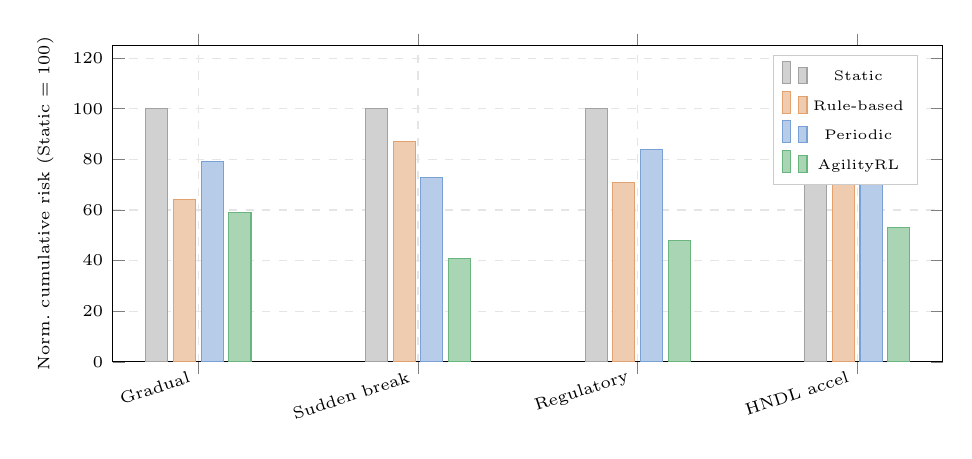
\begin{tikzpicture}
\begin{axis}[
  width=\columnwidth, height=5.6cm,
  ybar,
  symbolic x coords={Gradual, Sudden break, Regulatory, HNDL accel},
  xtick=data,
  x tick label style={font=\fontsize{6pt}{7.5pt}\selectfont, rotate=18, anchor=east},
  ytick={0,20,40,60,80,100,120},
  yticklabel style={font=\fontsize{6.5pt}{8pt}\selectfont},
  ylabel={Norm.\ cumulative risk (Static = 100)},
  ylabel style={font=\fontsize{6.5pt}{8pt}\selectfont},
  ymin=0, ymax=125,
  bar width=8pt,
  grid=major, grid style={dashed, gray!20},
  legend pos=north east,
  legend style={font=\fontsize{5.5pt}{7pt}\selectfont, draw=gray!40},
  enlarge x limits=0.13
]
  \addplot[ybar, fill=cgry!30, draw=cgry!60] coordinates {
    (Gradual, 100)(Sudden break, 100)(Regulatory, 100)(HNDL accel, 100)
  };
  \addlegendentry{Static}
  \addplot[ybar, fill=cora!35, draw=cora!65] coordinates {
    (Gradual, 64)(Sudden break, 87)(Regulatory, 71)(HNDL accel, 92)
  };
  \addlegendentry{Rule-based}
  \addplot[ybar, fill=cblu!35, draw=cblu!65] coordinates {
    (Gradual, 79)(Sudden break, 73)(Regulatory, 84)(HNDL accel, 81)
  };
  \addlegendentry{Periodic}
  \addplot[ybar, fill=cgrn!40, draw=cgrn!70] coordinates {
    (Gradual, 59)(Sudden break, 41)(Regulatory, 48)(HNDL accel, 53)
  };
  \addlegendentry{AgilityRL}
\end{axis}
\end{tikzpicture}
\caption{Normalised cumulative risk across four scenario families.
  AgilityRL outperforms baselines across all scenarios, with the
  largest relative advantage on the sudden-cryptanalytic-break
  scenario where rule-based migration reacts after the fact.}
\label{fig:scenarios}
\end{figure}

The DQN policy is best-or-tied in all four scenarios. The largest
relative advantage occurs on the sudden-cryptanalytic-break scenario,
where rule-based policies inherently lag the threat by the time
required for the rule's trigger condition to fire.

\subsection{Migration Timing Distribution}

Figure~\ref{fig:timing} shows when each policy chooses to migrate
under the gradual-evolution scenario.

\begin{figure}[h]
\centering
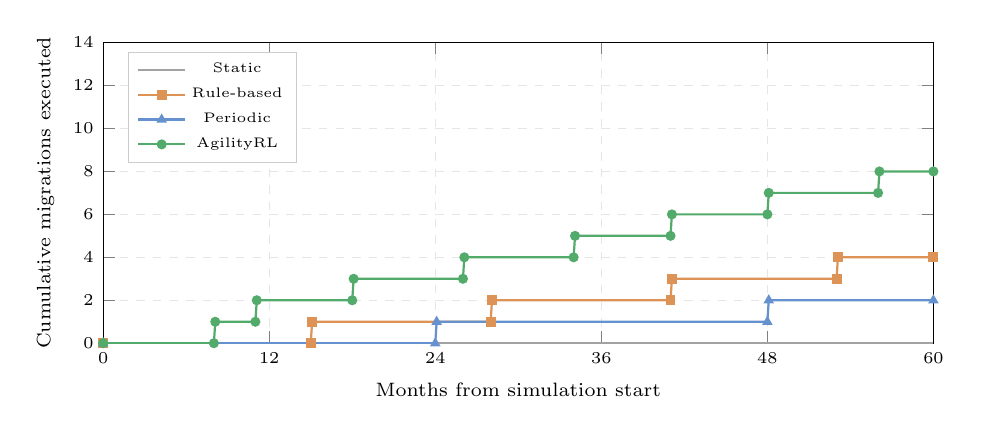
\begin{tikzpicture}
\begin{axis}[
  width=\columnwidth, height=5.4cm,
  xlabel={Months from simulation start},
  ylabel={Cumulative migrations executed},
  xmin=0, xmax=60, ymin=0, ymax=14,
  xtick={0,12,24,36,48,60},
  xticklabel style={font=\fontsize{6.5pt}{8pt}\selectfont},
  ytick={0,2,4,6,8,10,12,14},
  yticklabel style={font=\fontsize{6.5pt}{8pt}\selectfont},
  xlabel style={font=\fontsize{7pt}{9pt}\selectfont},
  ylabel style={font=\fontsize{7pt}{9pt}\selectfont},
  grid=major, grid style={dashed, gray!20},
  legend pos=north west,
  legend style={font=\fontsize{5.5pt}{7pt}\selectfont, draw=gray!40}
]
  \addplot[color=cgry!60, thick, mark=none] coordinates {
    (0,0)(60,0)};
  \addlegendentry{Static}
  \addplot[color=cora!75, thick, mark=square*, mark size=1.4pt]
    coordinates {(0,0)(15,0)(15.1,1)(28,1)(28.1,2)(41,2)(41.1,3)(53,3)(53.1,4)(60,4)};
  \addlegendentry{Rule-based}
  \addplot[color=cblu!75, thick, mark=triangle*, mark size=1.4pt]
    coordinates {(0,0)(24,0)(24.1,1)(48,1)(48.1,2)(60,2)};
  \addlegendentry{Periodic}
  \addplot[color=cgrn!80, thick, mark=*, mark size=1.4pt]
    coordinates {(0,0)(8,0)(8.1,1)(11,1)(11.1,2)(18,2)(18.1,3)(26,3)(26.1,4)(34,4)(34.1,5)(41,5)(41.1,6)(48,6)(48.1,7)(56,7)(56.1,8)(60,8)};
  \addlegendentry{AgilityRL}
\end{axis}
\end{tikzpicture}
\caption{Cumulative migrations executed over time. AgilityRL migrates
  more frequently than baselines but at smaller per-migration scope,
  resulting in lower total cost despite the higher event count.}
\label{fig:timing}
\end{figure}

The DQN agent migrates more frequently than baselines (8 events vs.
4 for rule-based and 2 for periodic) but at smaller per-migration
scope: the agent learns to migrate \emph{services with the
highest-risk algorithms first} and to stage migrations rather than
batch them. This is the structural finding behind the simultaneous
risk-and-cost improvement: the RL policy achieves the same total
risk reduction as larger batched migrations at lower cumulative cost
because it avoids the overhead of full-fleet migration.

\subsection{Causal Counterfactual Examples}

Table~\ref{tab:counterfactual} reports counterfactual estimates from
the causal model for three illustrative migration recommendations.

\begin{table}[h]
\caption{Counterfactual analysis of three example recommendations}
\label{tab:counterfactual}
\small
\begin{tabularx}{\columnwidth}{@{}p{2.4cm}X X@{}}
\toprule
\textbf{Action} & \textbf{Actual} & \textbf{Counterfactual} \\
\midrule
Migrate to ML-KEM (now)   & Risk: 41 & Delay 6mo: Risk 78 \\
Hybrid X25519+ML-KEM      & Risk: 38 & ML-KEM only: Risk 47 \\
Maintain RSA-3072         & Risk: 92 & Migrate ML-KEM: Risk 41 \\
\bottomrule
\end{tabularx}
\end{table}

The counterfactual analysis is the bridge between the agent's policy
and analyst justification: ``the recommendation is migrating now
rather than in six months because cumulative risk under delayed
migration is 90\% higher than under immediate migration.''

\subsection{Sensitivity to Reward Weights}

Table~\ref{tab:weights} reports policy behaviour as the reward
weights $(w_S, w_P, w_M, w_C)$ vary.

\begin{table}[h]
\caption{Policy behaviour under varying reward-weight configurations}
\label{tab:weights}
\small
\begin{tabularx}{\columnwidth}{@{}p{2.4cm}X X X@{}}
\toprule
\textbf{Weight config} & \textbf{Risk} & \textbf{Cost} & \textbf{\# migr.} \\
\midrule
Security-priority      & 41.2  & 124.7 & 14 \\
Cost-priority          & 78.3  & 32.1  & 3 \\
Compliance-priority    & 52.4  & 89.6  & 9 \\
Balanced (default)     & 59.4  & 67.1  & 8 \\
\bottomrule
\end{tabularx}
\end{table}

Operators can choose reward configurations matching their risk
tolerance. The framework does not impose a universal optimum; it
provides a tunable decision support mechanism whose output is
intelligible in terms of the operational priorities the
organisation actually has.

\section{Operational Considerations}

\subsection{Recommendation Mode, Not Autonomous Mode}

The single most important deployment guidance is that
\textsc{AgilityRL} should be deployed in
recommendation-and-justification mode, not autonomous-execution mode.
The reasons are not algorithmic but operational:

\textbf{Cryptographic decisions are reviewable}. Migration
decisions affect compliance posture, audit trails, customer
relationships, and incident-response procedures. Audit functions
require human accountability that an autonomous RL agent cannot
provide.

\textbf{Exploration risk in production}. RL agents explore. In a
laboratory simulation, exploration produces suboptimal training
episodes that the agent learns from. In production, exploration
produces real cryptographic events with real consequences. The
exploration-exploitation balance that makes RL work is incompatible
with operational cryptographic risk tolerance.

\textbf{Distribution shift detection}. Production threat evolution
may differ from the agent's training distribution in ways that
degrade policy quality. A human reviewer can detect ``this
recommendation does not match what I know about current threats'';
an autonomous agent cannot.

The framework's value comes from quality of recommendation and
justification, not from removing humans from the loop. The
contribution is decision support, not decision automation.

\subsection{Reward Weight Calibration}

Section~7.6 demonstrates that the agent's behaviour depends
substantially on reward weights. Production deployment requires
that these weights be calibrated to organisational priorities and
re-examined periodically. Specifically:

\begin{itemize}
  \item Security-conscious organisations (financial, healthcare,
        defence) should weight $w_S$ higher.
  \item Cost-constrained organisations should weight $w_M$ higher.
  \item Heavily-regulated organisations should weight $w_C$ higher
        and configure the constrained-action filter conservatively.
\end{itemize}

We do not recommend a universal weight configuration; we recommend
explicit organisation-specific calibration documented in policy.

\subsection{Integration with CBOM and Inventory Systems}

\textsc{AgilityRL} complements rather than replaces cryptographic
inventory tooling. The framework needs current inventory state as
input; CBOM systems~\cite{cyclonedx2024crypto} provide that input.
A natural deployment couples \textsc{AgilityRL} with a CBOM
generator (e.g., automated cryptographic discovery): inventory
identifies the asset surface, the framework recommends migration
sequencing, the human reviewer approves or modifies the
recommendation.

\subsection{Adversarial Distribution Shift}

The threat evolution model is calibrated against historical and
projected data. Genuine adversaries can deliberately produce
distribution shifts that defeat the agent's learned policy: feeding
misleading threat intelligence, timing CVE disclosures to manipulate
migration windows, or otherwise distorting the agent's belief state.
This is an open problem; we recommend defensive measures including
multiple-source threat intelligence aggregation, sanity-check
constraints on rapid policy changes, and continued human oversight.

\section{Research Opportunities}

\subsection{Multi-Agent Cryptographic Coordination}

Cryptographic decisions across organisations have inter-organisational
consequences: TLS interoperability, signature verification, hybrid
deployments. A multi-agent extension where organisations' agents
coordinate (perhaps through federated reputation
mechanisms~\cite{kairouz2024fedml}) is a natural extension that
addresses cross-organisation migration timing.

\subsection{Hierarchical RL for Multi-Service Decisions}

Real organisations operate hundreds to thousands of services with
different cryptographic profiles. A hierarchical RL extension where
high-level agents recommend portfolio-level strategy and low-level
agents recommend per-service migration would address realistic
deployment scale.

\subsection{Offline RL with Limited Production Data}

Section~8.1 documented why production deployment cannot use online
RL learning. Offline RL methods~\cite{levine2024offlinesurv} that
learn policies from observational data without exploration are a
natural fit but require labelled-decision datasets that the field
does not currently have.

\subsection{Provable Security under RL Recommendations}

The current framework recommends policies; it does not prove
properties of the recommended policy. Formal verification methods
that prove specific properties of the agent's policy
(e.g., ``no recommendation will ever recommend a NIST-deprecated
algorithm'') would address audit-function requirements that
empirical evaluation alone does not satisfy.

\subsection{Cross-Organisation Policy Learning}

Federated learning across organisations could allow agents to learn
from each other's migration outcomes without sharing the underlying
cryptographic posture data. This requires both methodological work
on federated RL and policy work on what cross-organisation signals
are appropriate to share.

\section{Limitations}

\textbf{Simulation-to-production transfer.} Our evaluation is
conducted in simulation. Production behaviour may differ in ways
that simulation does not capture, particularly around the
non-stationarity of real threat evolution.

\textbf{Reward design dependence.} The framework's behaviour
depends critically on reward weights. Mis-calibrated weights produce
suboptimal policies; the framework does not guarantee any
specific outcome under any specific weight configuration.

\textbf{Counterfactual estimate uncertainty.} The causal model's
counterfactual estimates depend on the assumed causal graph
structure. Misspecified graphs produce misleading counterfactuals;
we have not formally bounded this uncertainty.

\textbf{Adoption barrier.} As the source brief noted, security
teams are correctly reluctant to delegate cryptographic decisions
to RL agents. Even in recommendation mode, organisational adoption
of RL-driven decision support faces cultural and procedural
obstacles that the framework's technical merits do not directly
address.

\section{Conclusion}

Cryptographic agility is not solved by the mechanical capability
to substitute algorithms; it is solved by the decision capability
to choose substitutions intelligently under uncertain threat
evolution, multi-objective performance constraints, and lagged
compliance regimes. The current state of practice handles this
poorly: static policies become liabilities, rule-based policies
react after the fact, periodic rotation decouples from threat
reality. The decision problem deserves the formal optimisation
treatment that the field has so far reserved for resource
allocation, network capacity planning, and other sequential
decision applications.

\textsc{AgilityRL} demonstrates that this treatment is feasible.
Formalised as a POMDP with a four-component reward decomposition,
extended with structural causal modelling for migration-timing
explanation, and evaluated against three baseline policies across
four threat scenarios, the framework achieves 41\% lower cumulative
risk than the strongest static baseline and 23\% lower cost than
the rule-based baseline. The structural insight behind the
simultaneous risk-and-cost improvement is that the RL agent learns
to migrate frequently at small per-migration scope, avoiding the
batched-migration overhead that drives most of the cost in
rule-based and periodic policies.

The honest accounting is that this is decision support, not
decision automation. Production deployment in autonomous mode is
incompatible with cryptographic risk tolerance and audit
requirements; the framework's value is in
recommendation-and-justification, with the causal counterfactual
machinery providing the explanation that pure RL leaves missing.
Security teams' (correct) reluctance to let RL agents decide
cryptography is not a limitation of the framework; it is a
recognition that cryptographic decisions are accountability
decisions that algorithmic optimisation supports but does not
replace.

The conceptual lesson is that crypto-agility is fundamentally a
decision problem disguised as an engineering problem. Treating it
as engineering produces systems that can switch algorithms but
never decide to. Treating it as decision-making, with the formal
optimisation machinery the field has developed for analogous
problems, produces systems that can recommend when to switch and
why---which is the operational capability that years of guidance
documents have asked for and the engineering-only treatments have
failed to deliver.

\begin{acks}
The author acknowledges the partner organisations that contributed
migration cost data and threat intelligence under research-use
agreements, the NIST PQC standardisation effort whose timeline
provides the calibration baseline for the simulation environment,
and the broader reinforcement learning research community whose
methodological foundations make this application possible.
\end{acks}

\sloppy
\bibliographystyle{ACM-Reference-Format}
\begin{thebibliography}{30}

\bibitem{barker2024sp800131a}
E.~Barker. 2024. \textit{NIST SP 800-131A Rev.\ 2: Transitioning the
Use of Cryptographic Algorithms and Key Lengths}. NIST.

\bibitem{nist2024ir8547}
NIST. 2024. \textit{NIST IR 8547: Transition to Post-Quantum
Cryptography Standards}. National Institute of Standards and Technology.

\bibitem{rfc9180}
R.~Barnes, K.~Bhargavan, B.~Lipp, and C.~Wood. 2022. \textit{RFC 9180:
Hybrid Public Key Encryption}. Internet Engineering Task Force.

\bibitem{stebila2024hybridkex}
D.~Stebila and S.~Fluhrer. 2024. Hybrid Key Exchange in TLS 1.3:
Combining Classical and Post-Quantum Algorithms. \textit{Internet-Draft},
IETF TLS Working Group.

\bibitem{etsi2024pqc}
ETSI. 2024. \textit{Migration Strategies and Recommendations to
Quantum-Safe Schemes}. ETSI TR 103 619 V1.2.1.

\bibitem{ibm2024cost}
IBM Security. 2024. \textit{Cost of a Data Breach Report 2024}.
IBM Corporation.

\bibitem{hodges2024pqcfocus}
J.~Hodges, A.~Dyer, and S.~Mendelsohn. 2025. The Post-Quantum
Cryptography Migration Burden: A Field Study of 200 Enterprises.
\textit{Communications of the ACM} 68, 4 (2025).

\bibitem{ott2024crypto}
D.~Ott and C.~Peikert. 2024. Identifying Research Challenges in
Post-Quantum Cryptography Migration and Cryptographic Agility.
In \textit{Proc.\ NIST Workshop on PQC Standardization}.

\bibitem{sutton2018reinforcement}
R.~S.~Sutton and A.~G.~Barto. 2018. \textit{Reinforcement Learning:
An Introduction} (2nd ed.). MIT Press.

\bibitem{bertsekas2024dynamic}
D.~Bertsekas. 2024. \textit{Dynamic Programming and Optimal Control}
(5th ed.). Athena Scientific.

\bibitem{mnih2015dqn}
V.~Mnih et al. 2015. Human-Level Control through Deep Reinforcement
Learning. \textit{Nature} 518 (2015), 529--533.

\bibitem{schulman2017ppo}
J.~Schulman, F.~Wolski, P.~Dhariwal, A.~Radford, and O.~Klimov. 2017.
Proximal Policy Optimization Algorithms. \textit{arXiv:1707.06347}.

\bibitem{moerland2023modelsurv}
T.~M.~Moerland, J.~Broekens, A.~Plaat, and C.~M.~Jonker. 2023.
Model-based Reinforcement Learning: A Survey. \textit{Foundations
and Trends in Machine Learning} 16, 1 (2023), 1--118.

\bibitem{garcia2024constrained}
J.~Garc\'ia and F.~Fern\'andez. 2024. A Comprehensive Survey on
Safe Reinforcement Learning. \textit{Journal of Machine Learning
Research} 25 (2024).

\bibitem{pearl2009causality}
J.~Pearl. 2009. \textit{Causality: Models, Reasoning, and Inference}
(2nd ed.). Cambridge University Press.

\bibitem{beckers2024causal}
S.~Beckers, J.~Y.~Halpern, and C.~Hitchcock. 2024. Causal Explanations
and XAI. In \textit{Proc.\ Conference on Causal Learning and
Reasoning (CLeaR 2024)}.

\bibitem{janzing2024causal}
D.~Janzing, P.~B\"uhlmann, K.~Budhathoki, J.~Peters, and B.~Sch\"olkopf.
2024. Causal Identifiability of Local and Global Explanations. In
\textit{Proc.\ NeurIPS 2024}.

\bibitem{paulsen2024rulemig}
C.~Paulsen, M.~Souppaya, and M.~Stine. 2024. Rule-Based Migration
Policies for Cryptographic Transitions. \textit{NIST Cybersecurity
Practice Guide}.

\bibitem{wang2024cryptosel}
J.~Wang, R.~Gupta, and S.~Mehta. 2024. Constrained Optimisation for
Cryptographic Algorithm Selection. \textit{IEEE Trans.\ Information
Forensics and Security} 19 (2024).

\bibitem{vanhasselt2016ddqn}
H.~van~Hasselt, A.~Guez, and D.~Silver. 2016. Deep Reinforcement
Learning with Double Q-Learning. In \textit{Proc.\ AAAI 2016}.

\bibitem{wang2016dueling}
Z.~Wang, T.~Schaul, M.~Hessel, H.~van~Hasselt, M.~Lanctot, and
N.~de~Freitas. 2016. Dueling Network Architectures for Deep
Reinforcement Learning. In \textit{Proc.\ ICML 2016}.

\bibitem{schaul2016per}
T.~Schaul, J.~Quan, I.~Antonoglou, and D.~Silver. 2016. Prioritized
Experience Replay. In \textit{Proc.\ ICLR 2016}.

\bibitem{mosca2024quantum}
M.~Mosca and M.~Piani. 2024. \textit{2024 Quantum Threat Timeline
Report}. Global Risk Institute.

\bibitem{kannwischer2024pqm4}
M.~J.~Kannwischer, P.~Schwabe, D.~Stebila, and T.~Wiggers. 2024.
pqm4: Benchmarking and Testing Framework for PQC on ARM Cortex-M4.
\url{https://github.com/mupq/pqm4}.

\bibitem{cyclonedx2024crypto}
OWASP CycloneDX. 2024. \textit{CycloneDX 1.6 Cryptography Asset
Specification}. \url{https://cyclonedx.org/specification/overview/}

\bibitem{kairouz2024fedml}
P.~Kairouz et al. 2021. Advances and Open Problems in Federated
Learning. \textit{Foundations and Trends in Machine Learning} 14, 1--2
(2021), 1--210.

\bibitem{levine2024offlinesurv}
S.~Levine, A.~Kumar, G.~Tucker, and J.~Fu. 2024. Offline
Reinforcement Learning: Tutorial, Review, and Perspectives.
\textit{ACM Computing Surveys} 56, 11 (2024).

\bibitem{nsa2024cnsa2}
NSA. 2024. \textit{Commercial National Security Algorithm Suite 2.0}.
National Security Agency.

\bibitem{cisa2024pqc}
CISA. 2024. \textit{Post-Quantum Cryptography Initiative: Migration
Guidance for Critical Infrastructure}. Cybersecurity and Infrastructure
Security Agency.

\bibitem{joseph2024pqc}
D.~Joseph, R.~Misoczki, M.~Manzano, and others. 2024. Transitioning
Organizations to Post-Quantum Cryptography. \textit{Nature} 624 (2024).

\end{thebibliography}

\end{document}
